\begingroup
\section{加速器の原理}
本実験は京都大学小型中性子源KUANS(Kyoto University Accelerator-driven Neutron Source)で行った。本節ではKUANSについて説明する。
KUANSの性能は以下のようになっている。


\begin{table}[htb]\centering
\begin{tabular}{lcrr}
加速器&陽子線形加速器\\
加速粒子&陽子\\
最大加速エネルギー&3.5MeV\\
最大電流&100 $\mu$A \\
中性子発生ターゲット&Be\\
発生中性子エネルギー&keV~熱中性子(約2000m/s)\\
中性子減速材&ポリエチレン($10\times10\times10$ cm$^3$)
\end{tabular}
\end{table}
\begin{figure}[H]
\centering
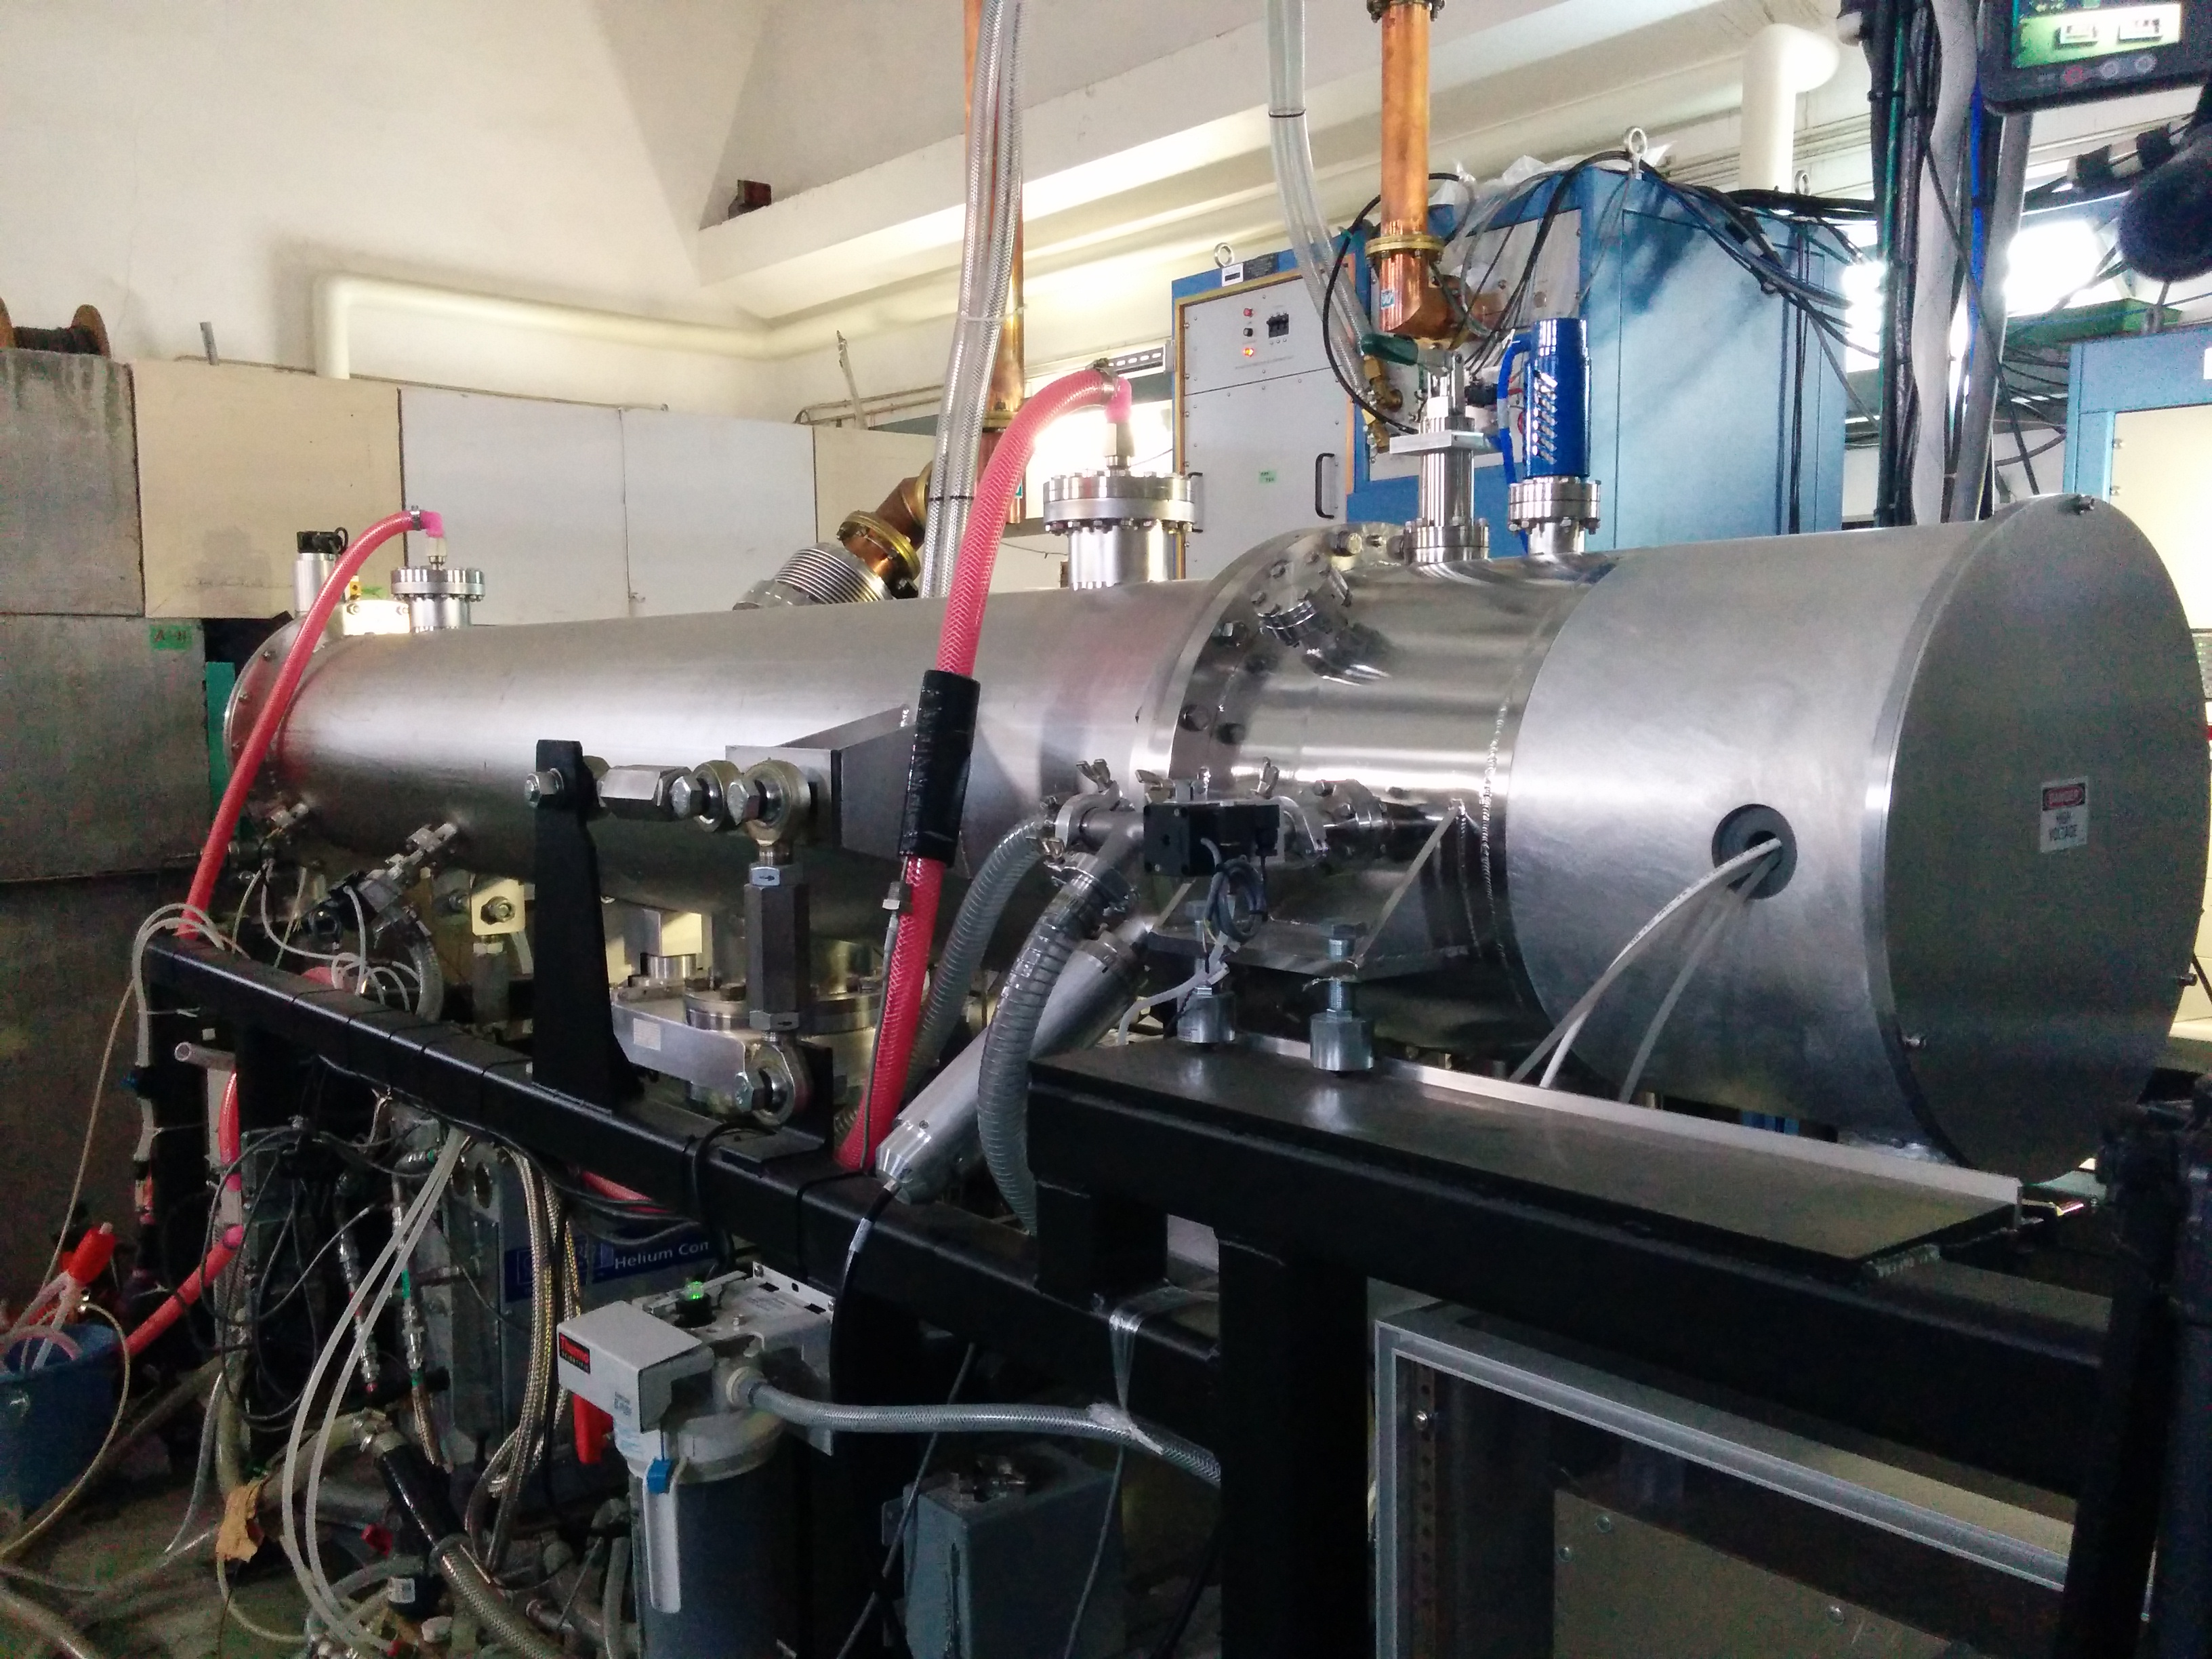
\includegraphics[width=9cm,height=6cm]{accelerator/accphoto.jpg}
\caption{陽子線形加速器}
\end{figure}

\subsection{中性子発生方法}
まず陽子線形加速器によって陽極で発生させた陽子を電圧で加速させ、シールド内に収められているBeターゲットへと衝突させる。
この際起こる以下の反応、
\begin{center}
$\ce{p} + \ce{^9Be} \to \ce{n} + \ce{^9B}$
\end{center}
によって中性子を発生させている。
しかしこのままの中性子は速すぎて実験に向かないので、KUANSでは減速材を用いて減速させ熱中性子とした後に、陽子ビームの向きと90$^{\circ}$をなす方向から取り出し、実験用中性子ビームとして利用している。
\newpage
\subsection{TOF(Time Of Flight)}
TOFとは一般的に粒子が加速されてから検出器に入るまでに要する時間のことである。
以降、本実験におけるTOFとは陽子線形加速器に電圧が印加されてから、発生した中性子が検出器に入るまでに要する時間のことを指すこととする。
このTOFは以下のように表せる。
\[
\mathrm{TOF}=T_f+T_o
\]
$T_f:減速材を出た中性子が検出器に達するまでに要する時間$\\
$T_o:補正する必要のあるオフセット$\\
本加速器においては、$T_o$は平均で約70$\mu$sであると報告されている。\cite{KUANS_yamashita}\\
実際に測定されたTOFから$T_m$の平均値70$\mu$sを引いたものを補正したTOFと呼び、$t$とする。
本実験では波長が重要な値となるので$t$から以下の式によって中性子の波長を算出した。
\begin{equation}
{\lambda}={\frac{ht}{md}}
\end{equation}
$d:減速材から検出器までの距離$

本実験においては約1100m/s、波長にして約3.5Åの範囲にある中性子を用いた。
\subsection{中性子のTOF分布}
\begin{figure}[H]
\centering
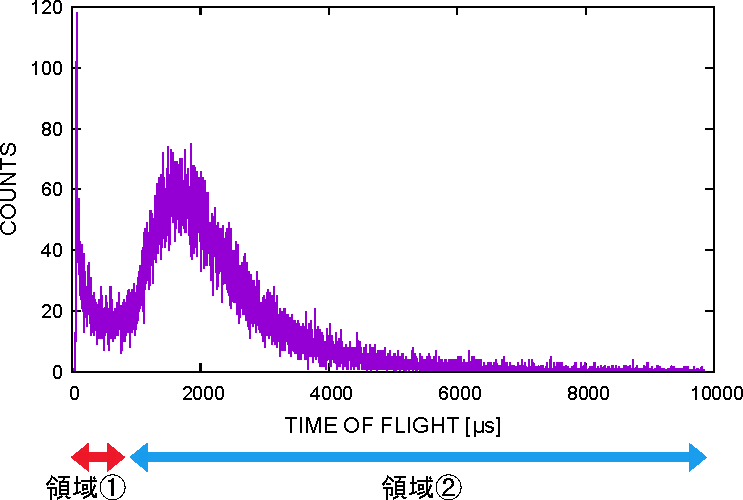
\includegraphics[width=9cm]{accelerator/TOF1.pdf}
\caption{実際に測定したTOF分布}
\end{figure}
領域①は減速材で熱平衡に達しなかった高速中性子に因る寄与であり、領域②は熱平衡に達した熱中性子に因る寄与である。
後者TOF分布$F(t)$は\begin{equation}F(t)\propto \frac{1}{t^{3}}\exp\left(-\frac{md^2}{2kTt^2}\right) \end{equation}で与えられる。

\paragraph{補足:中性子のフラックス} 
検出器に速度$v$で入射する中性子の数を考える。
検出器の表面の微小面積要素$dS$に垂直に$x$軸をとると、時間$dt$の間に速度{\bf $v$}=$(v_x,v_y,v_z)$で入射する中性子数$dN$は$n$を中性子数密度として
\begin{equation}
dN=nv_xdtf(v_x,v_y,v_z)dS
\end{equation}
で与えられる。

但し、$f(v_x,v_y,v_z)$は熱平衡にあり当方的な速度分布を持つ粒子が従う確率密度関数で以下の式で与えられる。
\begin{equation}
f(v_x,v_y,v_z)={\left(\frac{m}{2\pi kT}\right)}^{\frac{3}{2}}\exp\left\{-\frac{m}{2kT}(v^2_x+v^2_y+v^2_z)\right\} 
\end{equation}
後のため$f(v_x,v_y,v_z)$を極座標に変換すると、
\begin{equation}
f(v_x,v_y,v_z) \rightarrow f(v,\theta,\phi)={\left(\frac{m}{2\pi kT}\right)}^{\frac{3}{2}}v^2\exp\left(-\frac{mv^2}{2kT}\right)
\end{equation}
この微小面積要素$dS$に入射する粒子には様々な角度を持つものがあるので、$dS$に入射可能な角度範囲について積分すると、
\begin{eqnarray*}
 \iint dN\sin\theta d\theta d\phi &=&\iint nvdtf(v_x,v_y,v_z)\cos\theta \sin\theta d\theta d\phi dS \\ 
&=&ndtdS \hspace{-2pt}\iint \hspace{-2pt}{\left(\frac{m}{2\pi kT}\right)}^{\frac{3}{2}}v^3\exp\left(-\frac{mv^2}{2kT}\right)\cos\theta \sin\theta d\theta d\phi  \\
&=&ndtdS{\left(\frac{m}{2\pi kT}\right)}^{\frac{3}{2}} v^3\exp\left(-\frac{mv^2}{2kT}\right) \hspace{-2pt}\int \hspace{-2pt}\cos\theta\sin\theta d\theta \hspace{-2pt}\int \hspace{-2pt} d\phi \\
&=&Cv^3\exp\left(-\frac{mv^2}{2kT}\right)dtdS
\end{eqnarray*}
ここで$C$は速度には依らないが、検出器表面の場所には依存する関数である。

これより検出器にに入射する全粒子数$N$は、
\begin{eqnarray*}
N &=&
\iint_{検出器表面}Cv^3\exp\left(-\frac{mv^2}{2kT}\right)dSdt \\
&\propto& v^3\exp\left(-\frac{mv^2}{2kT}\right)
\end{eqnarray*}
この$v$を$t=d/v$で書き換えたものが先に示したTOF分布$F(t)$である。
\newpage
\subsection{LiM}
LiM(Lithium Monitor)はシールド内の減速材の後に置かれていて、ビームの一部を取り出して中性子ビーム強度を計測する役割を持つ。
このLiMの測定値と取り出した中性子ビーム強度は比例すると考えて本実験で規格化する際に用いた。
グラフは2/22のLiM測定値をある時間だけ抜き出したものである。但し、横軸は時刻である。
\begin{figure}[H]
\centering
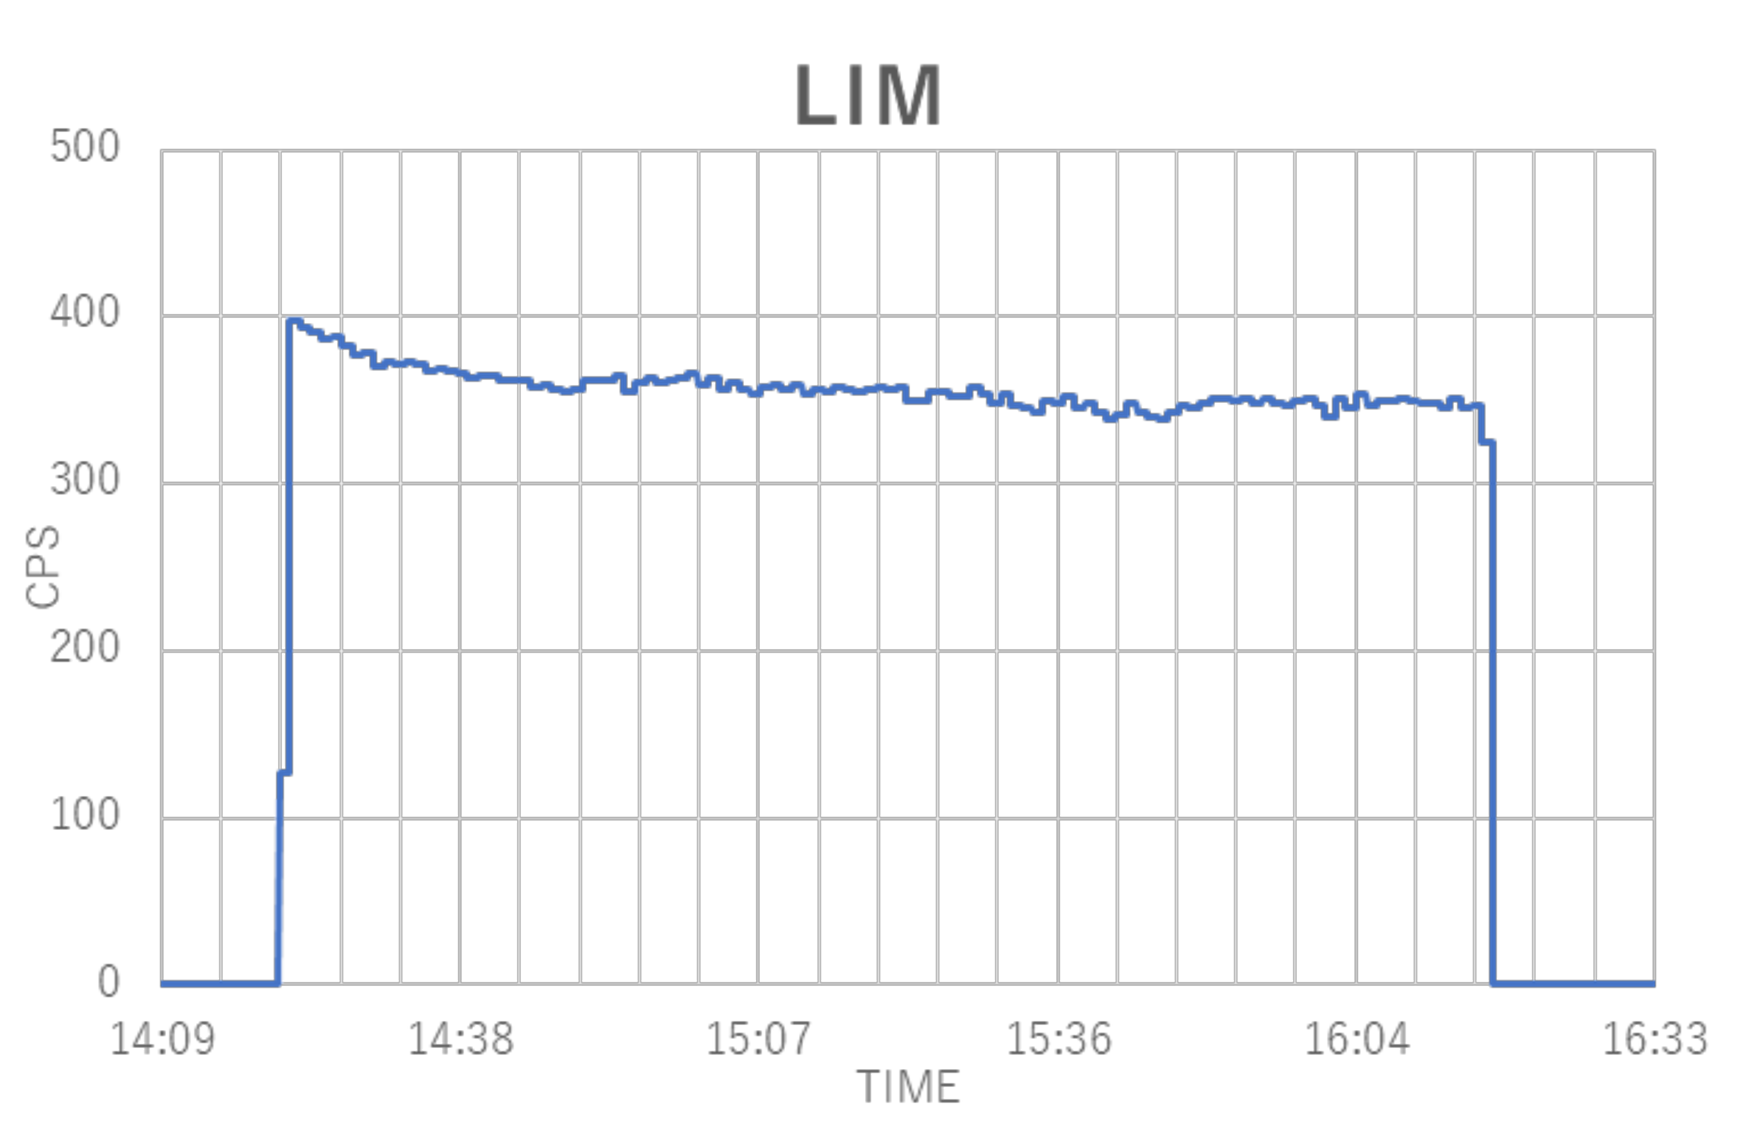
\includegraphics[width=9cm]{accelerator/LiM.pdf}\caption{LiMの時間変化}
\end{figure}
グラフを見ると分かるように本加速器は一定強度ではなく次第にビーム強度が低下し、ある値の周辺で変動する特徴があることが分かる。
\endgroup
